\documentclass[nonacm,acmtog]{acmart}
\usepackage{xcolor}
\usepackage{graphicx}
\usepackage{subcaption}
\newcommand{\todo}[1]{\textcolor{red}{\textbf{TODO}: #1}}
\newcommand{\TODO}{\textbf{\textcolor{red}{TODO}}}
\newcommand{\secref}[1]{\S\ref{#1}}


% Based off of Google Drive "Draft 1"

\newcommand{\dummyfig}[3]{
  \centering
  \fbox{
    \begin{minipage}[c][#3][c]{#2}
      \centering{#1}
    \end{minipage}
  }
}

% ==============================================================================
% ==[ Header information ]======================================================
% ==============================================================================

\title{Pre-Rigged Rappels for Safety and Speed}
\subtitle{CTAC-2019-03, Climbing Technical Advisory Committee}
%\author{Jeff Hunt}

% ==============================================================================
% ==[ Abstract ]================================================================
% ==============================================================================

\begin{abstract}
  Pre-rigged rappels are where the climbing team's rappel devices are all
  rigged for rappel before the first rappeller descends. The traditional
  method---not pre-rigging rappels---is where each climber attaches their
  rappel device to the rope, descends, and at the next anchor or on the ground,
  removes their rappel device before the next climber attaches their rappel
  device.

  In this report, CTAC recommends use of pre-rigged rappels for both
  Mountaineers field trips and climbing classes.  It describes not only the
  benefits but also the drawbacks of pre-rigged rappels in terms of safety,
  ease of use, and conditions under which is safe to use and finally, those
  where it should not be used.
\end{abstract}

\begin{document}
\maketitle

% ==============================================================================
\section{Introduction}
\label{sec:intro}
% ==============================================================================

  Pre-rigging a rappel is a technique that enables multiple climbers to
  simultaneously set up and check their rappels on the same rope system.  It
  has the potential to increase both climber safety and speed, by enabling
  partner checks and parallelizing the rigging process.  In scenarios where an
  experienced climber is descending with an inexperienced climber, it also
  allows the more experienced climber to set up the rappel for their
  novice---who may be uncomfortable in high angle terrain or unable to rig
  their own rappel with confidence---before descending first and providing
  further protection from below.

  Although pre-rigged rappels have become a popular technique in the guiding
  community, based on the experiences of this committee it has not seen as much
  popularity with private parties or climbing clubs, despite it's advantages in
  safety and speed.  We suspect this may be because publicly available material
  on this technique is simply less common compared to material discussing
  traditional rappelling techniques.  For example, one popular article on
  rappelling~\cite{www:aac-rappelling} only mentions pre-rigged rappels in
  passing, instead focusing the article on the more traditional rappel methods.

  The purpose of this report is to increase awareness of this technique and to
  advocate for its usage, especially by larger groups of climbers.
  \secref{sec:setup} begins by describing how to properly set up a pre-rigged
  rappel.  This is followed by discussion of the technique's strengths and
  limitations in \secref{sec:benefits} and \secref{sec:limitations}
  respectively.
  %\TODO \secref{sec:mountaineers} provides an overview of where and
  %how this technique is currently taught within the Mountaineers climbing
  %courses, and
  \secref{sec:reading} lists a few additional resources on this technique, and
  \secref{sec:conclusion} concludes this report with CTAC's recommendation of
  using this technique whenever possible.

% ==============================================================================
\section{Setting up and Using a Pre-Rigged Rappel}
\label{sec:setup}
% ==============================================================================

  First, each climber prepares for an extended rappel and secures their
  personal tether to the rappel anchor (for more information on the rigging of
  extended rappels, refer to CTAC 2019-02~\cite{ctac:2019-2}).  With personal
  tethers in place, all climbers can independently attach their own rappel
  device to the rope, with each device immediately below the previous.  Rappel
  devices set up in this fashion are said to be ``stacked''. The climber
  furtherest away from the anchor will be the first to descend, and should
  also attach an autoblock below their device to act as a backup, exactly like
  a standard rappel.  The final setup for two climbers looks like
  Figures~\ref{fig:final-setup} and \ref{fig:final-setup2}, though this setup
  can easily extend to three or more climbers as well.

  \begin{figure}
     \centering
     %\dummyfig{Final setup of the pre-rigged rappel.  Image forthcoming.}
     %  {2.5in}{1.5in}
     \begin{subfigure}[t]{0.22\textwidth}
        \centering
        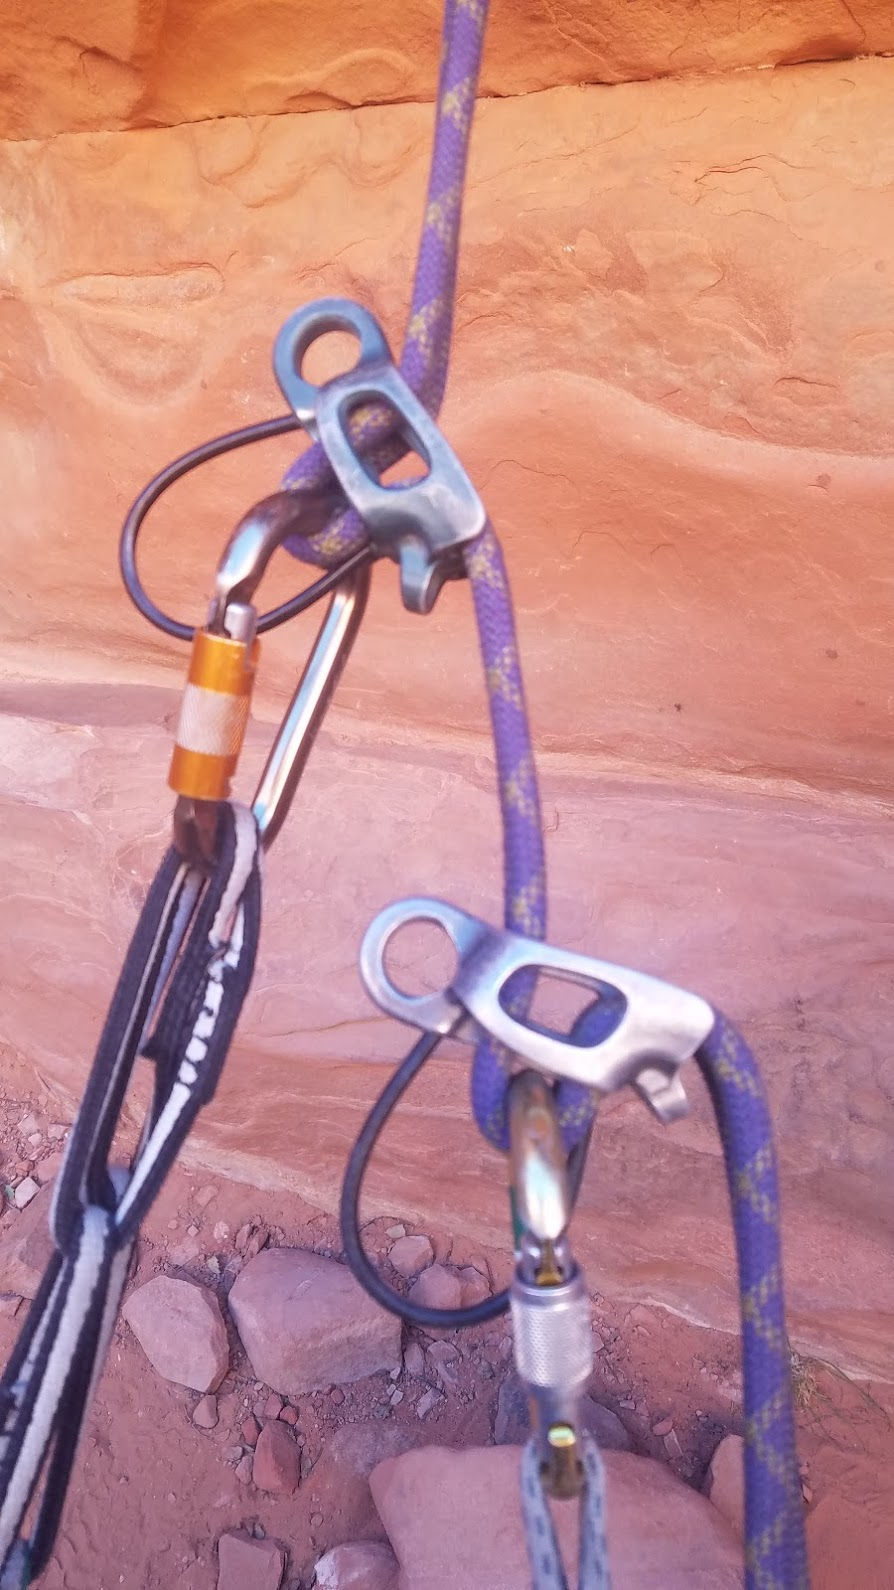
\includegraphics[width=1.5in]{images/setup1.jpg}
        \caption{Close-up of the stacked rappel devices.  The first to descend
           is rigged furthest from the anchor.}
        \label{fig:final-setup}
     \end{subfigure}
     \hspace{0.5cm}
     \begin{subfigure}[t]{0.22\textwidth}
        \centering
        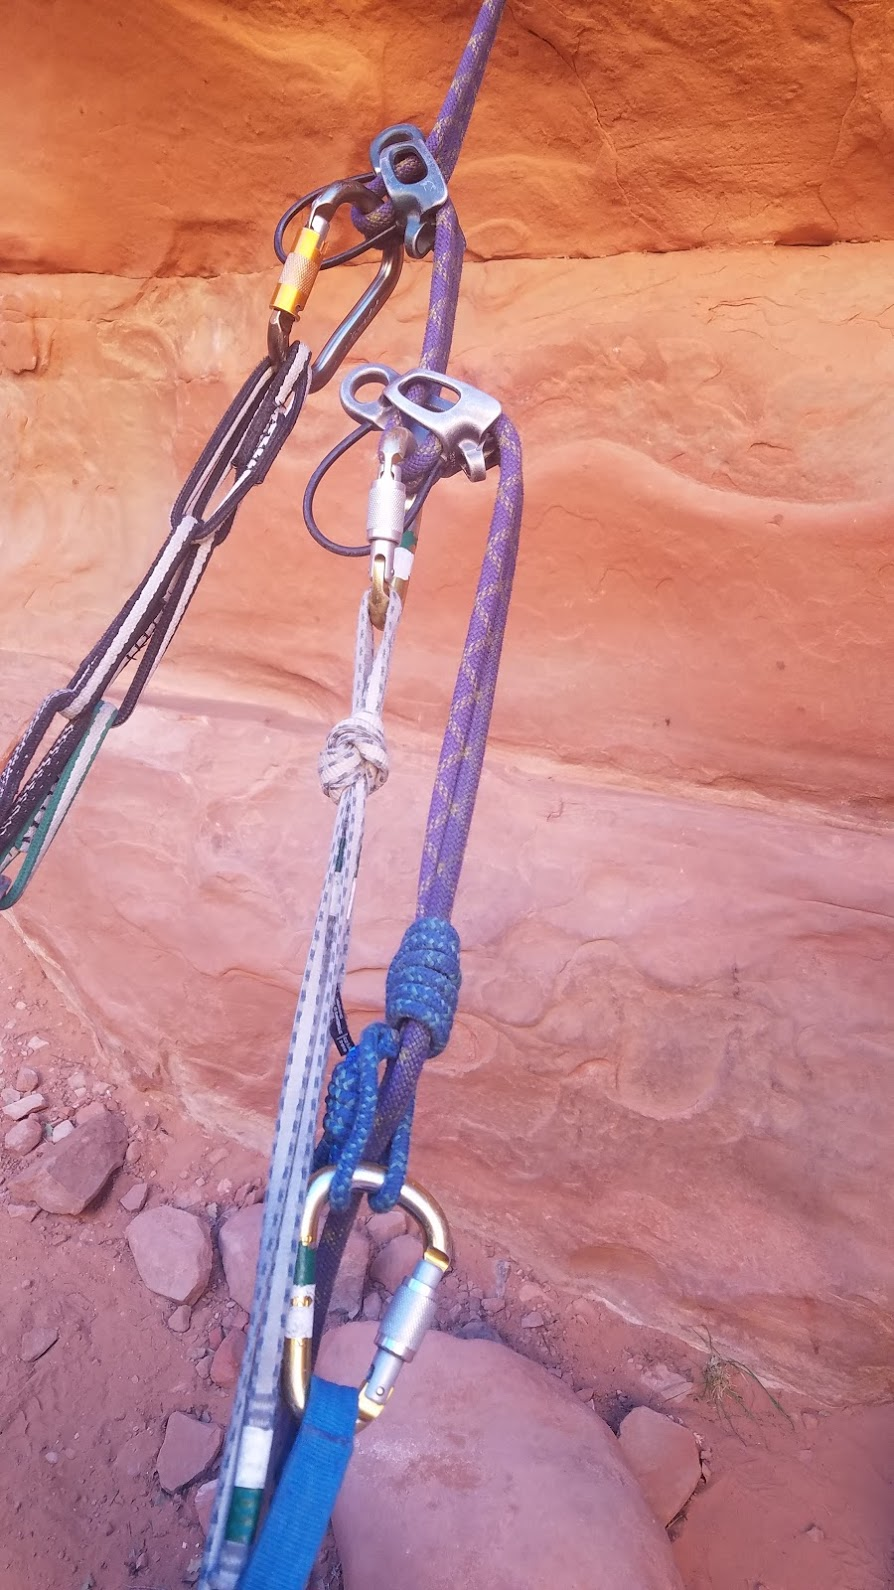
\includegraphics[width=1.5in]{images/setup2.jpg}
        \caption{The first to descend has also set up an autoblock backup.}
        \label{fig:final-setup2}
     \end{subfigure}
     \caption{Final setup of the pre-rigged rappel for two climbers.  Both
     climbers have their rappel devices on the rope, and the first climber to
     descend has an autoblock backup as well.}
  \end{figure}

  The rappel extensions in this setup also help ensure that climbers aren't too
  crowded at the station and can help isolate the climbers from any
  side-to-side motion of the rappel line as they await their turn to descend.

  For a more detailed, step-by-step visual walkthrough of setting up the pre-rigged
  rappel, the Seattle Mountaineers have produced a video~\cite[time
  4:55]{mountaineers:rappel-video} as well that walks through the entire process.

\subsection{Beginning the Descent}

  Once the pre-rigged rappels are set up as described above, each climber can
  visually inspect both their own rappel systems, as well as the systems of
  their climbing partners.  With cross-checks complete, the first climber to
  descend (the one whose rappel device is furtherest from the rappel anchor)
  can then test their setup by weighting the device and verifying its operation,
  before removing their tether and beginning their descent.

  The other climbers remain at the top of the pitch, attached to the rope via
  their rappel extensions and personal tethers.  Once the first rappeller goes
  off rappel, the next to descend can remove their tether from the anchor and
  begin their descent, optionally adding an autoblock to the rope as a backup,
  or relying on the previous rappellers to provide a fireman's belay from
  below.  Either form of backup is adequate, though the decision on which to
  use should be clearly communicated with all climbers before anyone descends.

%\subsection{Testing Before Use}

  % TODO: Move this paragraph to the next section?
  %
  %Multiple rappel devices attached to the rappel rope adds complexity that
  %could make visual assessment of the rigging more difficult especially in an
  %adverse environment such as low lighting, wind, and rain.  However, this is a
  %minor consideration with respect to the benefits of each climber cross
  %checking the other climbers' rigging as well and their own.

  %Pre-rigging the rappel does not change the ability to test the rappel before
  %use.  That is, with the personal tether attached and with slack, the climber
  %next up to rappel can test if the rappel device has been properly rigged
  %before removing the tether.  It is conceivable, however, that the act of
  %cross checking or assumed cross checking could engender complacency in
  %testing.  For this reason the CTAC recommendation that when using pre-rigged
  %rappels:

  %\begin{enumerate}
  %\item Cross checking is explicit with verbal confirmation.
  %\item Rappel rigging is tested with the personal tether attached and slack
  %  before the tether is removed.
  %\end{enumerate}


% ==============================================================================
\section{Benefits to Pre-rigging a rappel}
\label{sec:benefits}
% ==============================================================================

  Pre-rigging rappels in this fashion offers several benefits, broadly
  classified as either improving climber safety or group efficiency.

\subsection{Increased Climber Safety}

  Rappel accidents due to incorrectly attached rappel devices are,
  unfortunately, reported every year.  These types of climbing accidents can be
  prevented by testing a rappel setup before removing the tether, and by having
  one or more partners provide a visual cross-check each others device---a
  standard practice when it comes to belaying.

  However, with a traditional rappel, climbers set up their devices only when
  it is their turn to descend and the last to rappel is alone at the top of the
  pitch, making a partner check impossible.  Pre-rigged rappels, however, allow
  {\em all} climbers to have their systems be checked by other members of their
  group before anyone descends: a distinct advantage over standard rappels.

  Additionally, as described briefly in \secref{sec:intro}, pre-rigged rappels
  allow experienced climbers to help a novice setup their rappel, rather than
  leaving the novice to fend for themselves in a stressful and distracting
  environment.  The more experienced climber can verify the novice's setup,
  descend, find and prepare the next rappel station, and provide a fireman's
  belay to the novice from below.  The weight of the experienced climber on the
  rope will also prevent the novice climber from descending early, and at no
  point is the novice left alone with an unverified system.

\subsection{Increased Group Efficiency}
\label{sec:efficiency}

  Pre-rigged rappels can greatly enhance a climbing group's overall descent
  efficiency.  With standard rappels, each climber rigs and checks their rappel
  device immediately before descending.  Because this requires the rappel rope
  to be slack, they must wait to do this until the previous climber has
  completed their descent.  See the top of Figure~\ref{fig:schematic} for a
  visual representation of this, showing a timeline of the rigging, checking,
  and descending steps for three climbers (labelled A, B, and C in the figure).

  \begin{figure}[h]
   \includegraphics[width=0.45\textwidth]{images/schematic.pdf}
   \caption{Saving time with pre-rigged rappels, with three climbers labeled
   {\it A}, {\it B}, and {\it C}.  The top figure shows the steps for a
   traditional rappel; the middle figure shows the steps for a pre-rigged
   rappel as described in this document; the final figure highlights the
   additional time savings using the advanced technique described in
   \secref{sec:advanced}.  Because the rigging and checking of the rappel
   setups can all happen at the same time with the pre-rigged rappels, overall
   time spent rappelling on a pitch is reduced.} \label{fig:schematic}
  \end{figure}

  With pre-rigged rappels, however, the rigging and checking phases for all
  climbers can be performed at the same time; see the middle of the same figure
  for an example, where these blocks overlap.  This effect is described in an
  Alpine Savvy blog posting as follows~\cite{alpinesavvy:pre-rigged-rappels}:
  ``[Pre-rigged rappels] eliminate the downtime of waiting for climbers to rig
  the rappel one-by-one ...  The moment Rapper 1 goes off rappel, they quickly
  feed a couple meters of rope through their device and Rapper 2 can head down
  immediately. The movement of climbers down the rope is pretty much constant,
  with no waiting for someone to rig.''

  %Another efficiency gain comes when quads are used as the safety system at the
  %rappel chains---a technique that's useful in a multi-rappel setting.  Since
  %the final rappeller will be secured to the climbing rope with their rappel
  %device, they can tear down the quad while the second-to-laste climber is
  %descending.  This way they will be ready to descend as soon as the previous
  %climber reaches the next anchor.

  %  If the first rappeller is tied into the rope, the other end does not
  %  need a knot tied in. This is because the second rappeller keeps the rope
  %  locked off.  Not having a knot is one strand is one less thing to worry
  %  about potentially getting stuck. Also when rappelling on a clean wall and
  %  rope being pulled from the anchor above sails past the climbers, it is
  %  unnecessary to retrieve the end to tie a knot in the end.

\subsubsection{Additional Savings with Advanced Pre-Rigging}
\label{sec:advanced}

  Further efficiency can be gained by groups of experienced climbers if a
  slightly more advanced use of the pre-rigged rappel setup is used.  As long
  as there at least one climber remaining at the anchor, with their rappel device
  attached to the rope, two other climbers can safely rappel
  simultaneously---each climber using a single strand of the rope instead of
  two.  The pre-rigged rappel of the climber remaining at the top of the pitch
  locks the rope in-place, avoiding many of the risks associated with
  counter-balanced rappels: each rappeller can weight their own strand
  independently.  The additional time-savings afforded by this technique is
  highlighted in the bottom part of Figure~\ref{fig:schematic}, labeled
  ``Advanced Pre-rigged Rappels``.

  % TODO: Find a reference for this

% ==============================================================================
\section{Limitations}
\label{sec:limitations}
% ==============================================================================

  Despite the previously outlined advantages to pre-rigging rappels, there are
  also some disadvantages to this technique and environmental factors that
  should be taken in to consideration when deciding on a rappel strategy to
  employ with a group.  These will be discussed below.

\subsection{Disadvantages to Pre-Rigged Rappels}

  One disadvantage to this technique is that the first person down will be
  unable to perform a pull test on the rappel rope: the pre-rigged devices of
  the climbers remaining at the top of the pitch will prevent the rope from
  moving.  As such, if there is a risk that the rope will not pull cleanly from
  below, it is better to at least start with a standard rappel strategy and
  have the first person down make sure the rappel rope can be retrieved.  Once
  satisfied, the remaining climbers can then switch to pre-rigged rappels.

  Another disadvantage to this system is that if a rappeller is somehow
  incapacitated half-way down the descent (e.g., by rockfall), the remaining
  rappellers will not be able to easily exit the system.  The weight of the
  injured climber will effectively lock their pre-rigged devices in the system,
  requiring them to create a second tether and cut their original extension to
  escape the system.  Thus in situations where the risk of rockfall injury is
  high, it might be better to use standard rappel strategies instead.

\subsection{Inappropriate Environments}

   There are a few environments where pre-rigged rappels might be
   inappropriate.  For instance, if the rappel station is small or without a
   good stance, and the group is large (i.e., more than 3 climbers), it might
   be impractical for the entire group to approach the station and pre-rig.
   However, in these situations, some of the benefits of pre-rigged rappels can
   be gained by splitting the larger group in to two or more small groups, that
   can each employ the pre-rigged strategy independently.

   Additionally, stances where the rappel begins {\em above} the rappel station
   (i.e., ``sit and spin'' rappels) make the pre-rigged strategy impractical.
   For these types of anchors, a standard rappel strategy should be used
   instead.

\begin{comment}
% ==============================================================================
\section{Pre-Rigged Rappels and the Mountaineers}
\label{sec:mountaineers}
% ==============================================================================

  The Mountaineers' climbing classes teach pre-rigged rappels as follows:

  \begin{table}
  \begin{tabular}{|rll|}
    \hline
    \textbf{Branch} & \textbf{Class} & \textbf{Taught?} \\
    \hline\hline
    Everett    & Basic & No \\
               & Intermediate (LOR) & Considering \\
    \hline
    Bellingham & Basic & Demonstrated \\
               & Intermediate & Yes \\
    \hline
    Kitsap & --- & No \\
    \hline
    Olympia & --- & No \\
    \hline
    Seattle & Basic & No \\
            & Intermediate (rock, ice) & No \\
            & Advanced Alpine Rock     & Yes \\
    \hline
    Tacoma  & --  & No \\
    \hline
  \end{tabular}
  \caption{Current curriculum status of pre-rigged rappels in various courses
  at the Mountaineers branches}
  \end{table}
\end{comment}


\begin{comment}
% ==============================================================================
\section{CTAC Endorsement and Recommendation}
% ==============================================================================

  CTAC endorses the use of pre-rigged rappels whenever safe to do and when the
  conditions described in Downsides to Pre-rigging a rappel are not present.
  Furthermore, the CTAC majority opinion---with some dissenting opinions ---is
  that pre-rigging should be the standard operating procedure taught by The
  Mountaineers' climbing classes used on Mountaineers' field trips again under
  safe conditions.
\end{comment}

% ==============================================================================
\section{Further Reading}
\label{sec:reading}
% ==============================================================================

If the reader is interested in more discussion on this topic, there are a
number of reputable online and printed resources that cover this technique in
more detail.  Some of these are identified below; this is intended to be used
as a starting point and not as a comprehensive list of all sources.

\begin{itemize}
\item IFMGA guides Marc Chauvin and Rob Coppolillo describe the pre-rigged
   rappel in their 2017 book ``The Mountain Guide Manual'' \cite[pp. 182-183]{mgm}
\item IFMGA guide Jeff Ward recommends the use of pre-rigged and extended
   rappels in a 2016 blog posting for Rock and Ice's ``Ask the Masters'' blog
   series~\cite{www:ri-askthemaster-prerigged}
\item IFMGA guide Dale Remsberg describes and recommend pre-rigged rappels in
   the 2012 Climbing Magazine article titled ``Essential Skills: Pre-Rigging
   Rappels''~\cite{www:climbing-prerigged}.
\item A 2017 discussion on Mountain Project with input from recreational
   climbers describes using the pre-rigged rappels as a way to mitigate risk
   when rappelling with new climbers~\cite{www:mp-prerigged}
\end{itemize}

% ==============================================================================
\section{Conclusions}
\label{sec:conclusion}
% ==============================================================================

  In many situations, pre-rigged rappels offer climbers additional safety and
  efficiency benefits over the more standard one-at-a-time rappels.  These
  benefits make the pre-rigged rappels a valuable addition to the set of
  strategies that can be used by the private and club-climbing communities.
  Pre-rigged rappels are especially useful for multipitch climbs, where there
  are multiple back-to-back rappels, and when there is a mix of strong and weak
  climbers on the team.

  In most situations, overall group safety can be increased through the use of
  pre-rigged rappels.  However, as with all climbing techniques and skills,
  there are a few limitations to its use, and it should not be used blindly for
  all rappelling situations.  It is up to the individual climbers to assess
  their specific situation and to understand the hazards and trade-offs
  employing this technique.

\bibliographystyle{plain}
\bibliography{../ctac.bib}
\end{document}

% ==============================================================================
% ==[ Workspace ]===============================================================
% ==============================================================================

